\documentclass{article}

% Language setting
% Replace `english' with e.g. `spanish' to change the document language
\usepackage[english]{babel}

% Set page size and margins
% Replace `letterpaper' with `a4paper' for UK/EU standard size
\usepackage[letterpaper,top=2cm,bottom=2cm,left=2cm,right=2cm,marginparwidth=1.75cm]{geometry}

% Useful packages
\usepackage[colorlinks=true, allcolors=blue]{hyperref}
\usepackage{graphicx} 
\usepackage{booktabs}

\usepackage{fancyhdr}
\pagestyle{fancy}
\fancyhf{}
\rhead{For John-Doe - Jhon\_Doe\@gmail.com}
\lhead{Cupboard model from www.website.net}
\rfoot{Page \thepage}


\title{Your new cabinet is here!}
\author{Design from www.website.net}

\begin{document}
\maketitle

\begin{figure}[h!]
    \centering
    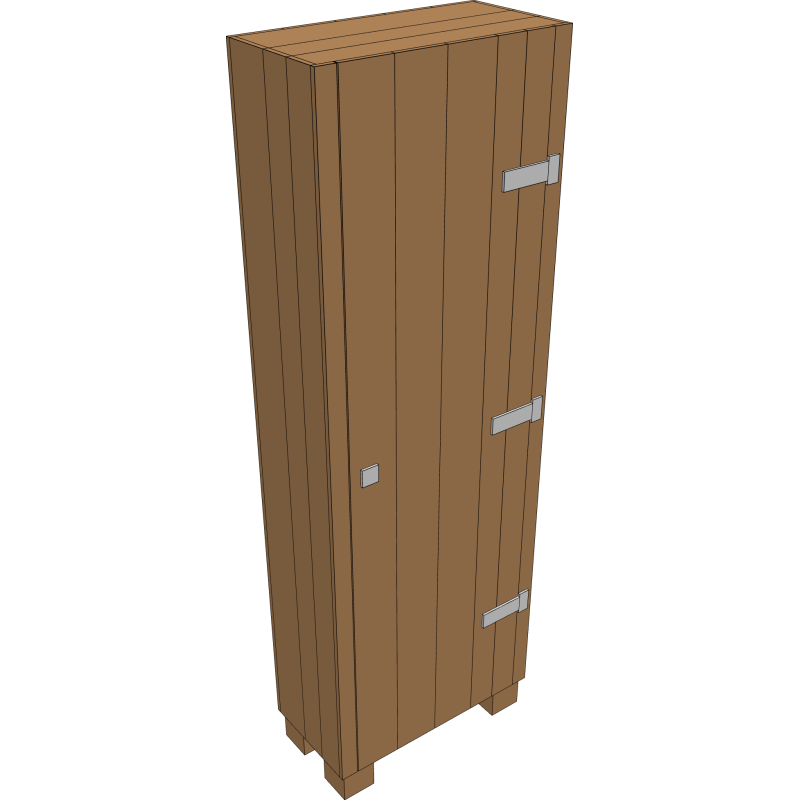
\includegraphics[width=\textwidth]{scene 12 - compleet.png}
\end{figure}

\clearpage
\newpage

\tableofcontents

\clearpage
\newpage

\section{Introduction}

Thank you for your confidence in this manual. This document describes step-by-step how to assemble the cabinet you specified. This chapter briefly explains the different parts of the assembly process. The shopping list is discussed in chapter two. The third chapter focuses on assembling your new closet. All measurements described in this manual are in centimeters unless otherwise indicated. \\

Despite the fact that a lot of attention has been paid to this model, it is always possible that there are errors. We therefore recommend that you carefully read the document for errors or inconsistencies before purchasing parts. If you come across errors, could you let us know? We will then correct the error and you will receive your money back for both this manual and the modified assembly manual. We are \underline{not} responsible for any damages (both physical and financial) resulting from following this manual. \\

The cabinet designed by us has the following exterior dimensions and floors: \\

\begin{table}[h!]
\centering
\caption{Basis afmetingen kast}
\begin{tabular}{rrr}
\toprule
 breedte &  hoogte &  diepte \\
\midrule
     300 &     300 &      50 \\
\bottomrule
\end{tabular}
\end{table}
 

\begin{center}
\textbf{We wish you lots of fun with this assembly and your new cabinet!}
\end{center}

\begin{figure}[h!]
    \centering
    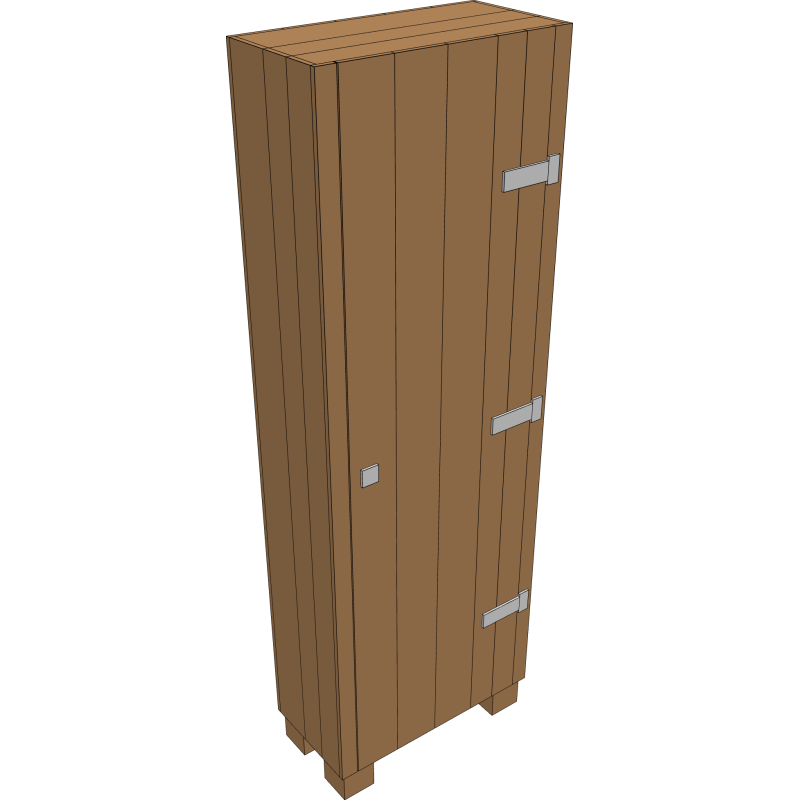
\includegraphics[width=0.7\textwidth]{scene 12 - compleet.png}
\end{figure}

\clearpage
\newpage

\section{Shopping list}

To assemble the cabinet you will need the following materials and tools. \\

\subsection{Materials}

First of all, the planks and beams. You can use both planed and unplaned wood for this. Unplaned wood is cheaper, but note that the dimensions of these planks and beams can differ. It may therefore be necessary to remove extra wood during construction due to the deviating dimensions.

\begin{table}[h!]
\centering
\caption{Required planks and beams for construction}
\begin{tabular}{lrrrr}
\toprule
 type &  width &  thickness &  length &  ammount \\
\midrule
plank &     20 &          2 &     300 &       23 \\
 beam &      3 &          3 &     300 &        6 \\
\bottomrule
\end{tabular}
\end{table}


The following properties have been drawn up for the legs. You are free to choose any leg shape here as long as the number and height of the chosen legs correspond to the table below.

\begin{table}[h!]
\centering
\caption{Eigenschappen van kastpoten}
\begin{tabular}{rr}
\toprule
 aantal poten &  hoogte \\
\midrule
            8,0 &     5,0 \\
\bottomrule
\end{tabular}
\end{table}


The table of the required screws is shown below. We recommend that you use wood screws with an M4 diameter. \href{https://www.amazon.nl/gp/product/B00B214ZLQ/ref=ppx_yo_dt_b_asin_title_o07_s00?ie=UTF8&psc=1}{These M4 wood screws} (figure \ref{fig:schroeven}) are a good option. Please note that the length of the screw may be different for your cabinet. Select a screw that has a length close to the 'max length'. Do not take longer screws, they will go through the wood which does not give a nice finish.

\begin{table}[h!]
\centering
\caption{Benodigde schroeven voor constructie}
\begin{tabular}{lrr}
\toprule
{} &  max lengte &  aantal \\
\midrule
Schroef 1 &           5 &       0 \\
Schroef 2 &           3 &       0 \\
Schroef 3 &           4 &       0 \\
\bottomrule
\end{tabular}
\end{table}


\begin{figure}[h!]
    \centering
    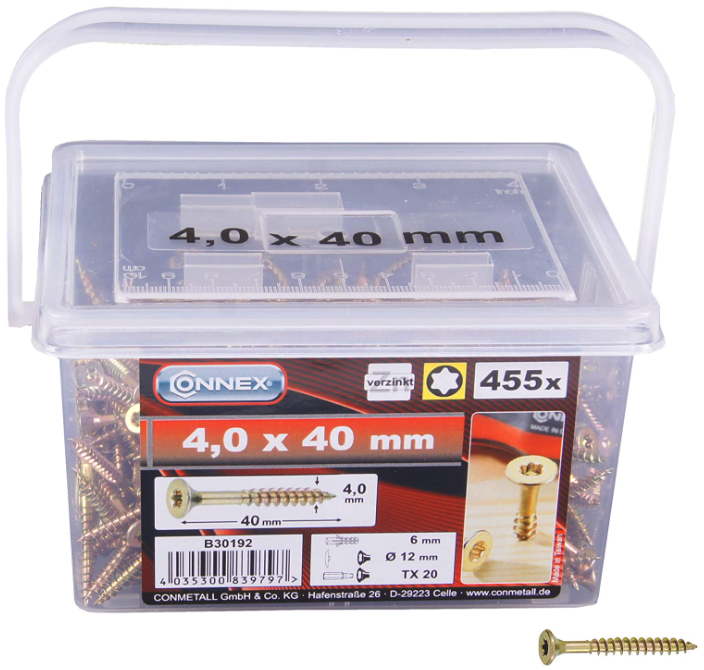
\includegraphics[width=0.3\textwidth]{schroeven.png}
    \caption{Connex M4 Screws from Amazon}
    \label{fig:schroeven}
\end{figure}

\clearpage
\newpage

Finally, additional metal parts are needed for the construction. For the corner frames it is recommended to select one with 4 holes and a maximum width of 3 centimeters. These ensure a strong connection. \href{https://www.amazon.nl/Connex-HVG2400-voordeelpak-hoekverbinder-verzinkt/dp/B00J7L2ET8/ref=sr_1_9?__mk_nl_NL=%C3%85M%C3%85%C5%BD%C3%95% C3%91&crid=22ED59WFFPB0Z&keywords=corner connector&qid=1660427081&sprefix=corner connector%2Caps%2C85&sr=8-9}{These corner connections} (figure \ref{fig:hoeken}) are a good option. For the hinges and locks you are of course completely free to choose which one best suits your personal taste.

\begin{table}[h!]
\centering
\caption{Overige benodigde onderdelen voor constructie}
\begin{tabular}{llr}
\toprule
{} & gaten raamwerk &  aantal \\
\midrule
Hoek verbinding &              4 &       0 \\
Scharnier       &         max 10 &       0 \\
Slot            &          max 4 &       0 \\
\bottomrule
\end{tabular}
\end{table}


\begin{figure}[h!]
    \centering
    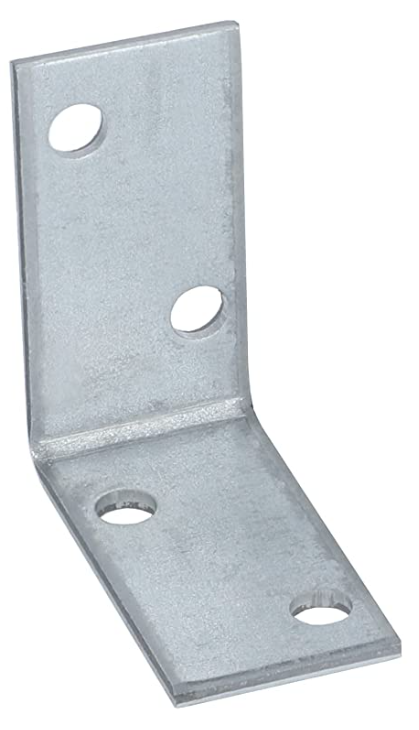
\includegraphics[width=0.2\textwidth]{hoeken.png}
    \caption{Connex corner connections from Amazon}
    \label{fig:hoeken}
\end{figure}

\subsection{Tools}

The tools below are required to build this cabinet.

\begin{itemize}
    \item Pencil
    \item Sawtable
    \item Screwmachine
    \item Measuring tape
\end{itemize}

In addition, the following items are optional. If you are using wood that has not been planed, the parts below are particularly recommended as unplaned planks can have significant variations in thickness, width and straightness.

\begin{itemize}
    \item Jigsaw
    \item Scrape
    \item Tri square
\end{itemize}

\begin{center}
    \textit{Tip: Don't have tools at hand? Then try searching for it via \href{https://www.peerby.com/}{Peerby}!}
\end{center}

\clearpage
\newpage

\section{Cutting list}

\subsection{Planks and beams length}

The table below shows how the beams and planks \underline{to length} are cut. The minimum required number of planks and beams has been calculated, if you do not follow this saw list you may run out of wood.

\begin{table}[h!]
\centering
\caption{Zaaglijst lengte per plank, Totaal 55 planken}
\begin{tabular}{lrrrr}
\toprule
{} &     1 &    2 &    3 &  aantal \\
\midrule
1 &  90,0 & 90,0 & 90,0 &       3 \\
2 & 295,0 &  0,0 &  0,0 &      40 \\
3 & 296,0 &  0,0 &  0,0 &      12 \\
\bottomrule
\end{tabular}
\end{table}


\begin{table}[h!]
\centering
\caption{Sawlist length per beam, Totalling to 6 beams}
\begin{tabular}{lrrrrrr}
\toprule
{} &     1 &    2 &    3 &    4 &    5 &  ammount \\
\midrule
1 &  40,0 & 40,0 & 40,0 & 40,0 & 40,0 &        1 \\
2 &  90,0 & 90,0 & 40,0 & 40,0 & 40,0 &        1 \\
3 & 281,0 &  0,0 &  0,0 &  0,0 &  0,0 &        4 \\
\bottomrule
\end{tabular}
\end{table}


\subsection{Planks and beams width}

Now that the planks and beams have been sawn, some of the planks also need to be adjusted in width and length. Select the planks from the list and cut them to the required width. \\

\begin{center}
    \textit{Tip: write the measurements on the planks and beams with a pencil for quick reference later!}
\end{center}

\begin{table}[h!]
\centering
\caption{Partlist beams and planks}
\begin{tabular}{lrrrr}
\toprule
 type &  width &  thickness &  length &  ammount \\
\midrule
 beam &    3,0 &        3,0 &    40,0 &        8 \\
 beam &    3,0 &        3,0 &    90,0 &        2 \\
 beam &    3,0 &        3,0 &   281,0 &        4 \\
plank &    7,5 &        2,0 &   285,0 &        2 \\
plank &   12,2 &        2,0 &   285,0 &        2 \\
plank &   13,0 &        2,0 &    96,0 &        4 \\
plank &   13,0 &        2,0 &   285,0 &        4 \\
plank &   20,0 &        2,0 &    85,0 &        3 \\
plank &   20,0 &        2,0 &    96,0 &        6 \\
plank &   20,0 &        2,0 &   285,0 &       10 \\
\bottomrule
\end{tabular}
\end{table}


\clearpage
\newpage

\section{Assembly}

\subsection{Step 1 - Bottom and feet}

First of all, you construct the base of the cabinet. The table below shows the materials required for this step. In this table, the first row is the cabinet legs and the next are the shelves for the bottom.

\begin{table}[h!]
\centering
\caption{Stap 1 Samenstelling voeten en bodem}
\begin{tabular}{rrrr}
\toprule
 lengte &  breedte &  dikte &  aantal \\
\midrule
    5,0 &      5,0 &    5,0 &       8 \\
  396,0 &      8,0 &    2,0 &       2 \\
  396,0 &     10,0 &    2,0 &       1 \\
\bottomrule
\end{tabular}
\end{table}


The image below shows how the legs are attached to the shelves. The order of laying the boards is irrelevant. To fix the legs in the planks, use \textbf{two screws} per foot. For this you step use \textbf{screw 1} as indicated in table 4 of chapter 2.

Sizes shown are from the left side of the cabinet to the beginning of the leg. Legs are placed at the ends of the cabinet in width. The image below is depicted extra large in the appendix.

\begin{figure}[h!]
    \centering
    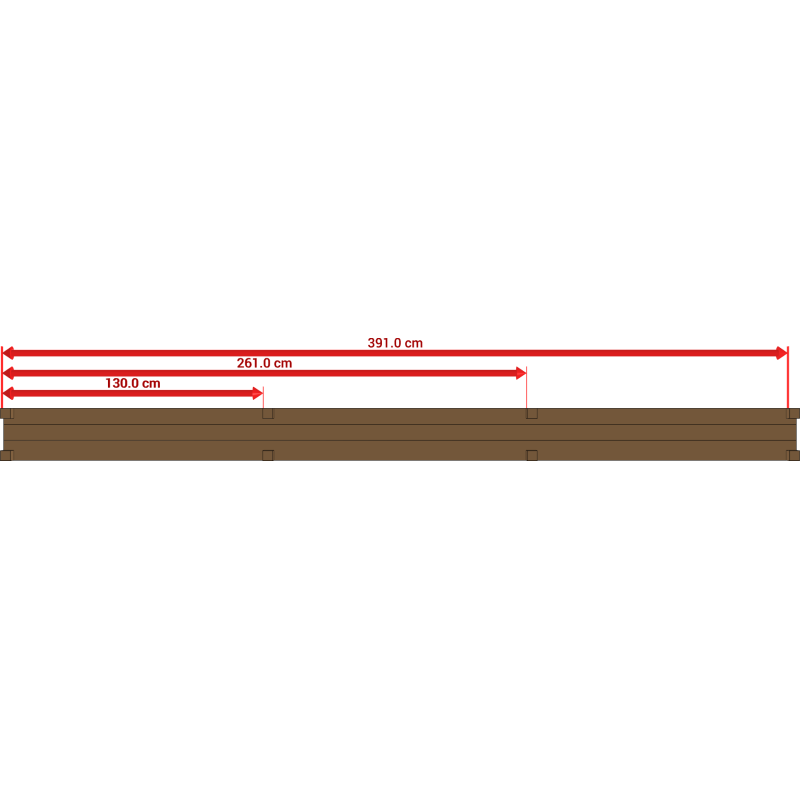
\includegraphics[width=0.8\textwidth]{scene 1 - bottom.png}
    \caption{Bottom view cabinet}
    \label{fig:stap 1}
\end{figure}

\clearpage
\newpage

\subsection{Step 2 - Bottom and ribs}

Now screw the ribs onto the cabinet. The table below shows the materials required for this step.

\begin{table}[h!]
\centering
\caption{Step 2 Assembly step 1 and bottom rib}
\begin{tabular}{rrrr}
\toprule
 length &  width &  thickness &  ammount \\
\midrule
   40,0 &    3,0 &        3,0 &        2 \\
\bottomrule
\end{tabular}
\end{table}


The image below shows how the ribs are attached to the planks. To fasten the ribs in the planks, use \textbf{one screw per plank per rib}. For this you use \textbf{screw 1} as indicated in table 4 of chapter 2. This screw first goes through the plank and then ends in the beam.

Sizes shown are from the left side of the cabinet to the start of the ribs. The vertical distance shown ensures that the ribs are placed in the middle of the planks. The image below is depicted extra large in the appendix.

\begin{figure}[h!]
    \centering
    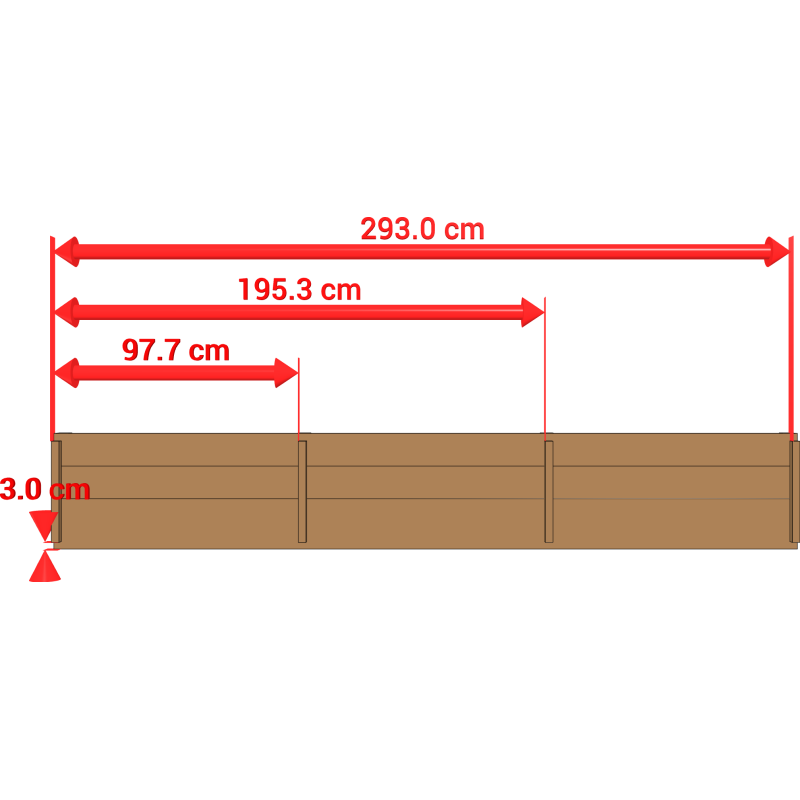
\includegraphics[width=0.8\textwidth]{scene 2 - bottom rib.png}
    \caption{Ribs on cabinet}
    \label{fig:stap 2}
\end{figure}

\clearpage
\newpage

\subsection{Step 3 - Ladder frame}

Then you construct the ladder frame. The table below shows the materials required for this step. With this list you make all ladder frames for your closet, make an equal distribution of the beams for each ladder frame in your closet.

\begin{table}[h!]
\centering
\caption{Step 3 Ladder frame}
\begin{tabular}{rrrr}
\toprule
 length &  width &  thickness &  ammount \\
\midrule
   40,0 &    3,0 &        3,0 &       16 \\
   94,7 &    3,0 &        3,0 &        9 \\
  291,0 &    3,0 &        3,0 &        8 \\
\bottomrule
\end{tabular}
\end{table}


The figure below shows how the vertical ribs are attached to the horizontal beams. To fix the ribs in the beams, use a corner connection per corner with \textbf{four screws} per connection and place it at the location of the green arrow. For this you use \textbf{screw 2} as indicated in table 4 of chapter 2.

Sizes shown are placed from the top of the frame to the start of the rib. The image below is depicted extra large in the appendix.

\begin{figure}[h!]
    \centering
    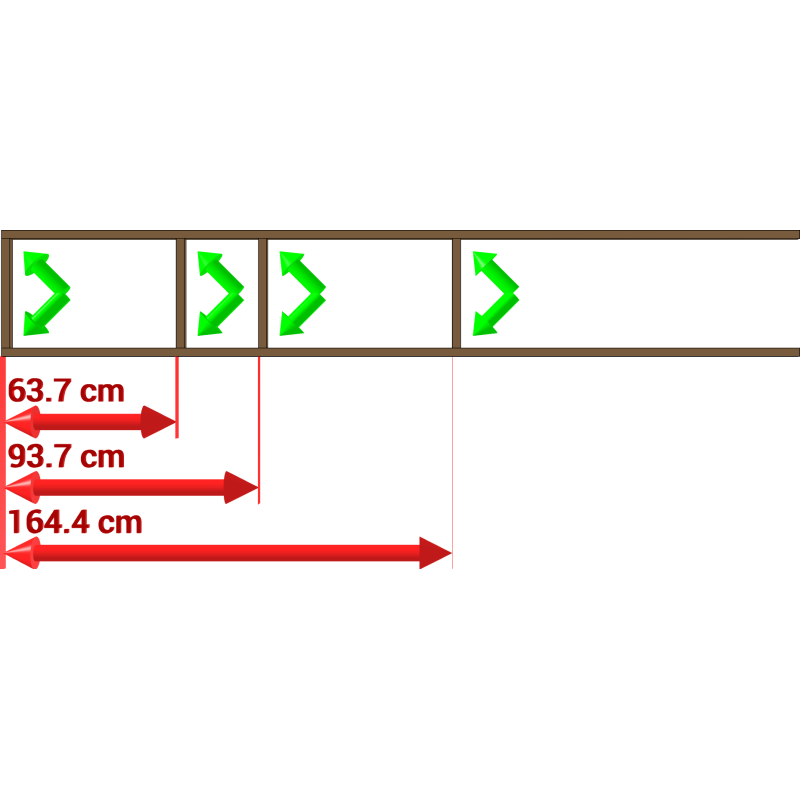
\includegraphics[width=0.8\textwidth]{scene 3 - ladder.png}
    \caption{Ladder frame}
    \label{fig:stap 3}
\end{figure}

\clearpage
\newpage

\subsection{Step 4 - Ladder frame on bottom}

Then connect the ladder to the cabinet base.

The image below shows how the ladder is attached to the frame. To fasten the ladder to the ribs, use a corner connection per corner with \textbf{four screws} per connection and place it at the location of the green arrow. For this you use \textbf{screw 2} as indicated in table 4 of chapter 2.
The image below is depicted extra large in the appendix.

\begin{center}
\textit{Note that in this step the construction can be unstable, so make sure the ladders don't fall over! By using good corner joints you ensure that the construction remains stable in this step.}
\end{center}

\begin{figure}[h!]
    \centering
    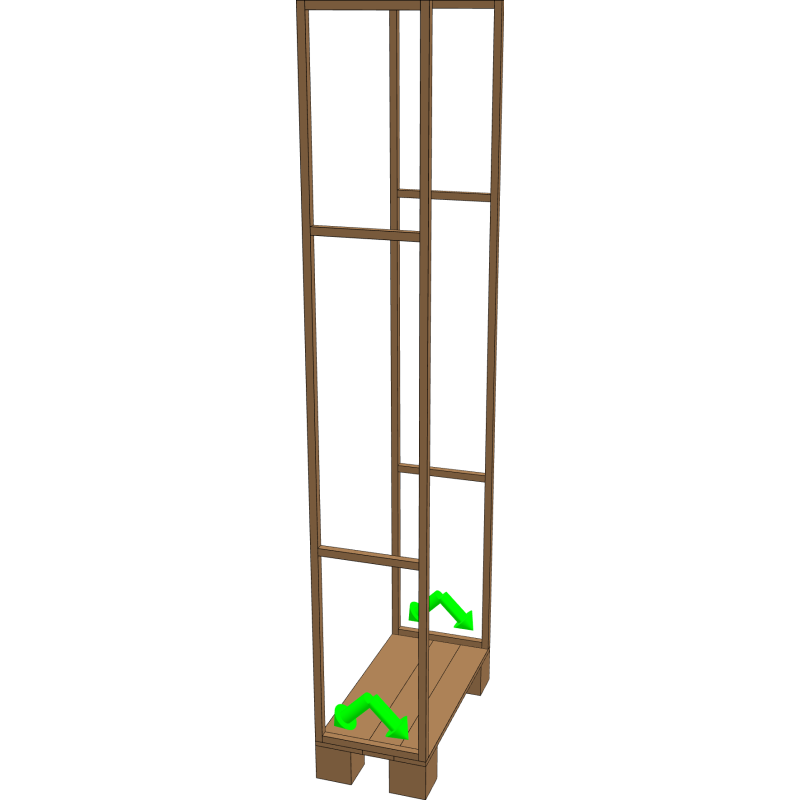
\includegraphics[width=0.8\textwidth]{scene 4 - geraamte.png}
    \caption{Ladder frame on bottom}
    \label{fig:stap 4}
\end{figure}

\clearpage
\newpage

\subsection{Step 5 - Backside ribs}

Then you construct the rear rib system of the cabinet. The table below shows the materials required for this step.

\begin{table}[h!]
\centering
\caption{Stap 5 Samenstelling stap 2, stap 3 en achter rib}
\begin{tabular}{rrrr}
\toprule
 lengte &  breedte &  dikte &  aantal \\
\midrule
  128,0 &      3,0 &    3,0 &       3 \\
\bottomrule
\end{tabular}
\end{table}


The image below shows how the ribs are connected to the rear ribs. To fasten the ribs to the back rib, use a corner connection per corner with \textbf{four screws} per connection and place it at the location of the green arrow. For this you use \textbf{screw 2} as indicated in table 4 of chapter 2.

Measurements shown are from the top of the horizontal ribs in the ladder to the top of the back rib. The size of the distance is equal to the thickness of the plank in the recess. The images below are depicted extra large in the appendix.

\begin{figure}[h!]
    \centering
    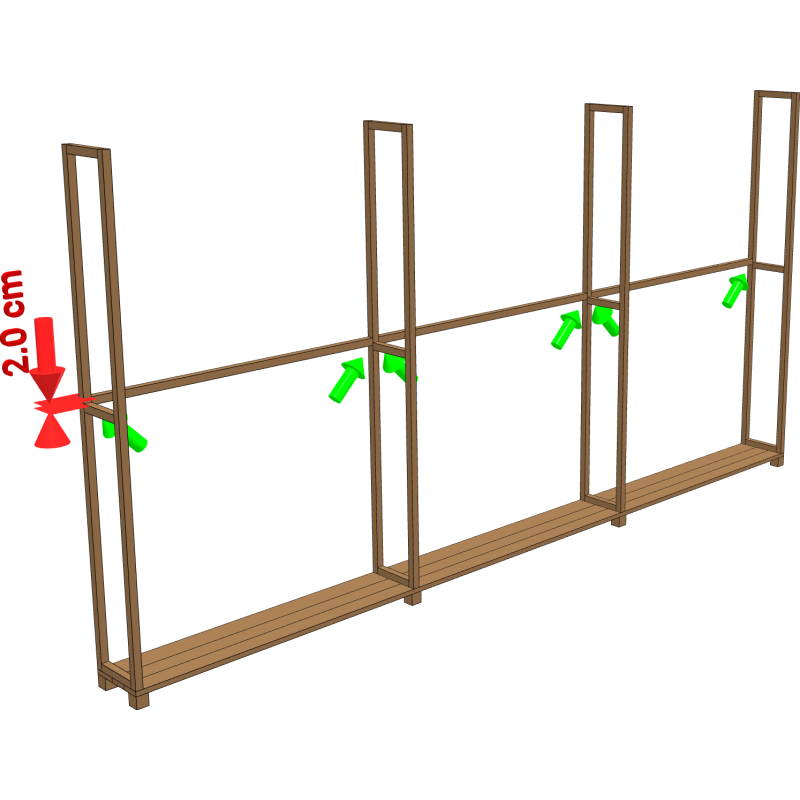
\includegraphics[width=0.8\textwidth]{scene 5 - achterrib a.png}
    \caption{Backside rib global}
    \label{fig:stap 5a}
\end{figure}

\begin{figure}[h!]
    \centering
    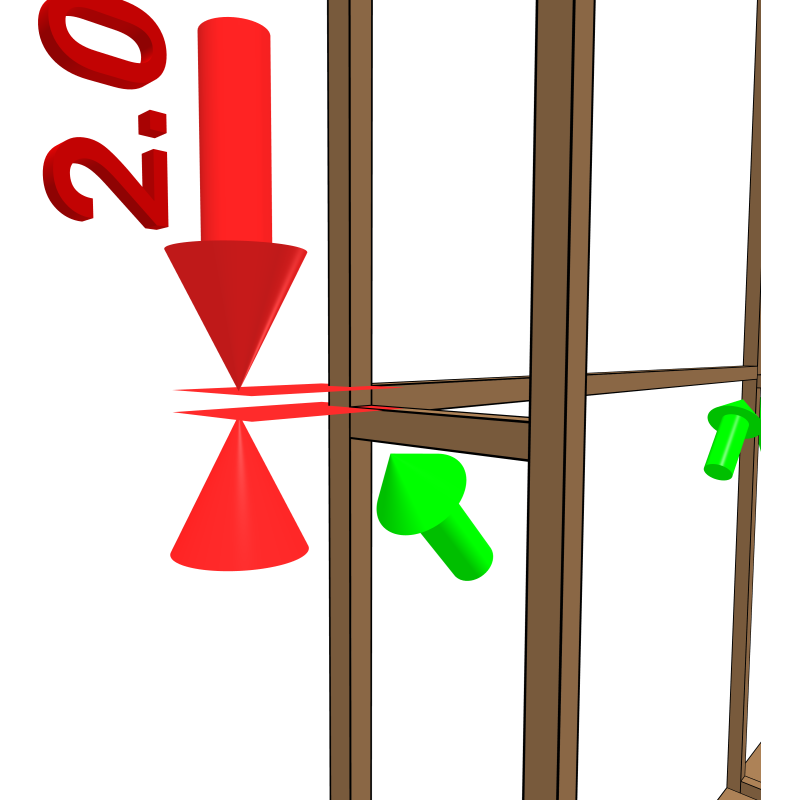
\includegraphics[width=0.8\textwidth]{scene 5 - achterrib b.png}
    \caption{Backside rib local}
    \label{fig:stap 5b}
\end{figure}

\clearpage
\newpage

\subsection{Step 6 - Decking}

Now it's time to place the decking of your closet. The table below shows the materials required for this step. With this list you make all the decking for your closet, make an equal distribution of the shelves for each floor in your closet.

\begin{table}[h!]
\centering
\caption{Step 6 Assembly step 5 and platforms}
\begin{tabular}{rrrr}
\toprule
 length &  width &  thickness &  ammount \\
\midrule
   96,0 &   20,0 &        2,0 &        4 \\
\bottomrule
\end{tabular}
\end{table}


The image below shows how the planks are connected to the ribs of the ladder. The order of laying the boards is irrelevant. To fix the planks to the ribs, screw each plank \textbf{with one screw} for each location where it comes into contact with a rib of the ladder. For this you use \textbf{screw 1} as indicated in table 4 of chapter 2. This screw first goes through the plank and then ends in the beam.

Measurements shown are from the top of the horizontal ribs in the ladder to the top of the back rib. The images below are depicted extra large in the appendix.

\begin{figure}[h!]
    \centering
    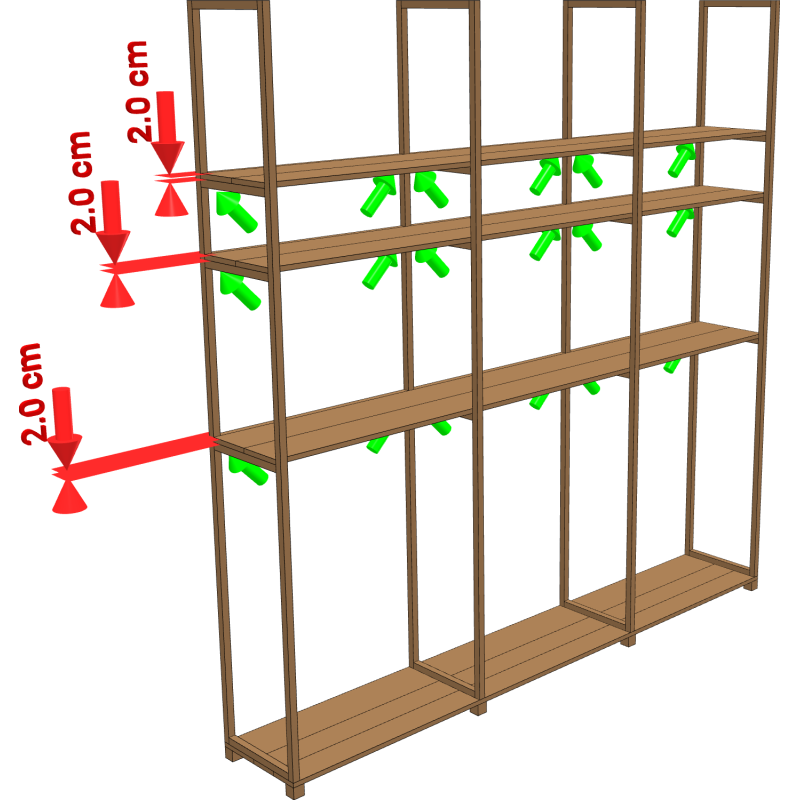
\includegraphics[width=0.8\textwidth]{scene 6 - vlonders a.png}
    \caption{Decking global}
    \label{fig:stap 6a}
\end{figure}

\begin{figure}[h!]
    \centering
    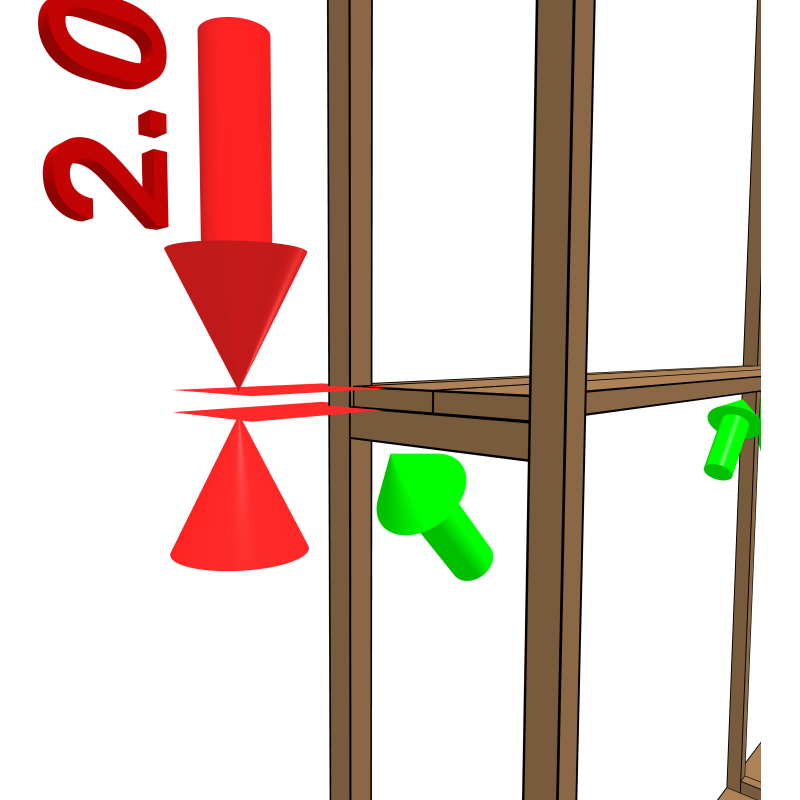
\includegraphics[width=0.8\textwidth]{scene 6 - vlonders b.png}
    \caption{Decking local}
    \label{fig:stap 6b}
\end{figure}

\clearpage
\newpage

\subsection{Step 7 - Top cover}

Now it's time to build the cabinet top cover. The table below shows the materials required for this step.

\begin{table}[h!]
\centering
\caption{Stap 7 Samenstelling stap 6 en bovenkant}
\begin{tabular}{rrrr}
\toprule
 lengte &  breedte &  dikte &  aantal \\
\midrule
  296,0 &     13,0 &    2,0 &       2 \\
  296,0 &     20,0 &    2,0 &       1 \\
\bottomrule
\end{tabular}
\end{table}


The image below shows how the planks are connected to the ribs of the ladder. To fix the planks to the ribs, screw each plank \textbf{with one screw} for each location where it comes into contact with a rib of the ladder. For this you use \textbf{screw 1} as indicated in table 4 of chapter 2. This screw first goes through the plank and then ends in the beam.

The images below are depicted extra large in the appendix.

\begin{figure}[h!]
    \centering
    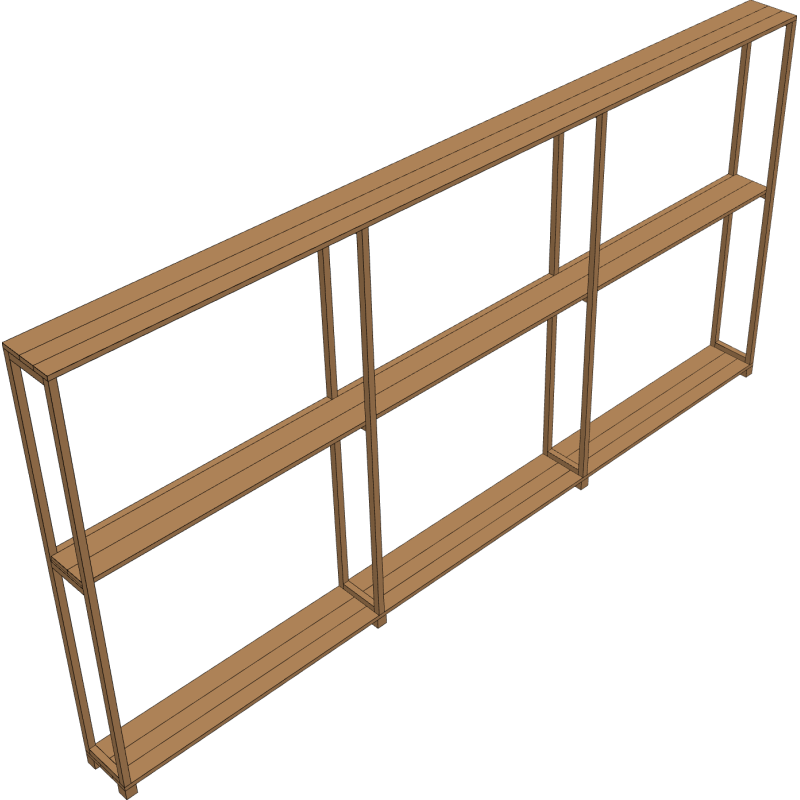
\includegraphics[width=0.8\textwidth]{scene 7 - boven.png}
    \caption{Topside cabinet}
    \label{fig:stap 7}
\end{figure}

\clearpage
\newpage

\subsection{Step 8 - Sides}

Then the sideboards of the cabinet are constructed. The table below shows the materials required for this step. With this list you make all the sides for your cabinet, make an equal distribution of the shelves for the left and right side.

\begin{table}[h!]
\centering
\caption{Stap 8 Samenstelling stap 7 en zeiden}
\begin{tabular}{rrrr}
\toprule
 lengte &  breedte &  dikte &  aantal \\
\midrule
  195,0 &      8,0 &    2,0 &       4 \\
  195,0 &     10,0 &    2,0 &       2 \\
\bottomrule
\end{tabular}
\end{table}


The image below shows how the planks are connected to the horizontal bars of the ladder. The order of placing the shelves is irrelevant. To secure the planks to the beams, screw each plank \textbf{with one screw} for each location where it comes into contact with a horizontal rib of the ladder. For this you use \textbf{screw 1} as indicated in table 4 of chapter 2. This screw first goes through the plank and then ends in the beam. The distances shown indicate the height for inserting the screws at the level of the ribs. These are shown relative to the underside of the cabinet (bottom of the legs).

The images below are depicted extra large in the appendix.

\begin{figure}[h!]
    \centering
    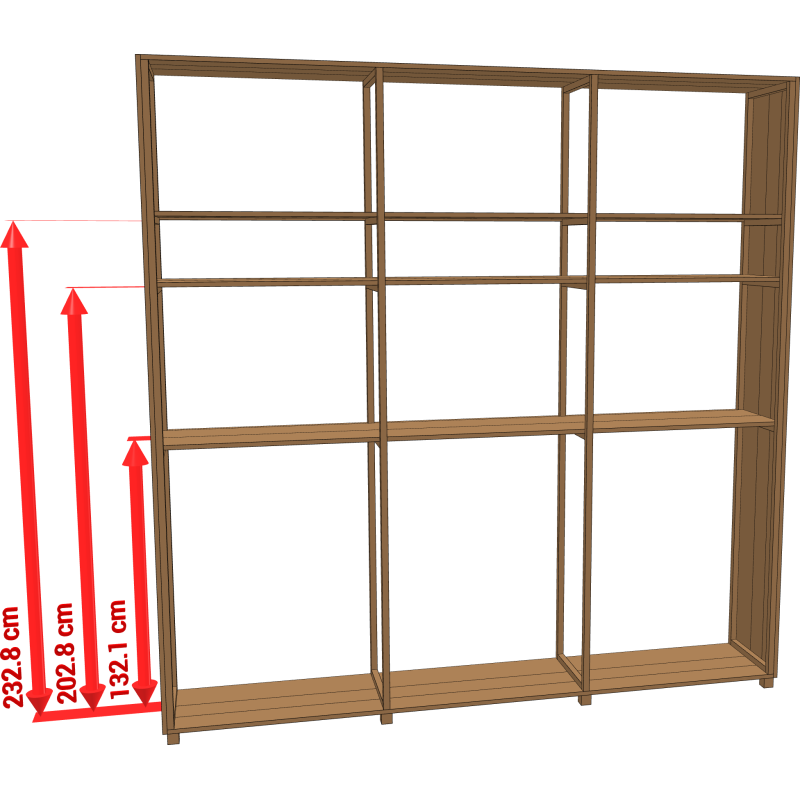
\includegraphics[width=0.8\textwidth]{scene 8 - links_rechts.png}
    \caption{Sides cabinet}
    \label{fig:stap 8}
\end{figure}

\clearpage
\newpage

\subsection{Step 9 - Backside}

Then the back of the cabinet is constructed. The table below shows the materials required for this step.

\begin{table}[h!]
\centering
\caption{Step 9 Assembly step 8 and back side}
\begin{tabular}{rrrr}
\toprule
 length &  width &  thickness &  ammount \\
\midrule
  494,0 &   20,0 &        2,7 &       10 \\
\bottomrule
\end{tabular}
\end{table}


The image below shows how the shelves are connected to the horizontal rear ribs of the cabinet. The order of placing the shelves is irrelevant. To secure the shelves to the beams, screw each shelf \textbf{with one screw} for each location where it comes into contact with a horizontal back rib of the cabinet. For this you use \textbf{screw 1} as indicated in table 4 of chapter 2. This screw first goes through the plank and then ends in the beam. The distances shown indicate the height for inserting the screws at the level of the rear ribs. These are shown relative to the underside of the cabinet (bottom of the legs).

The images below are depicted extra large in the appendix.

\begin{figure}[h!]
    \centering
    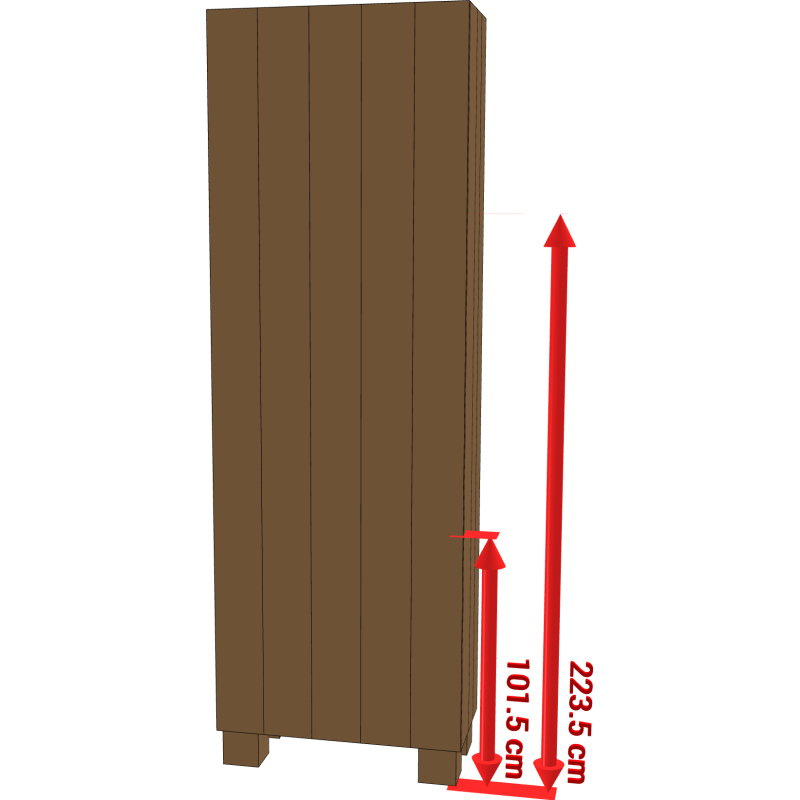
\includegraphics[width=0.8\textwidth]{scene 9 - achterkant.png}
    \caption{Backside cabinet}
    \label{fig:stap 9}
\end{figure}

\clearpage
\newpage

\subsection{Step 10 - Door frame}

Now the door frames of the cabinet are constructed. The table below shows the materials required for this step.

\begin{table}[h!]
\centering
\caption{Stap 10 Samenstelling en deurpost(en)}
\begin{tabular}{rrrr}
\toprule
 lengte &  breedte &  dikte &  aantal \\
\midrule
  195,0 &      7,5 &    2,0 &       4 \\
\bottomrule
\end{tabular}
\end{table}


The image below shows how the shelves are connected at the front of the cabinet. To fix the planks to the beams, screw each plank with \textbf{one screw} for each location at the level of a horizontal rib of the ladder. For this you use \textbf{screw 1} as indicated in table 4 of chapter 2. This screw first goes through the plank and then ends in the beam. The distances shown indicate the distance from the outside of the cabinet to the start of the shelf.

The images below are depicted extra large in the appendix.

\begin{figure}[h!]
    \centering
    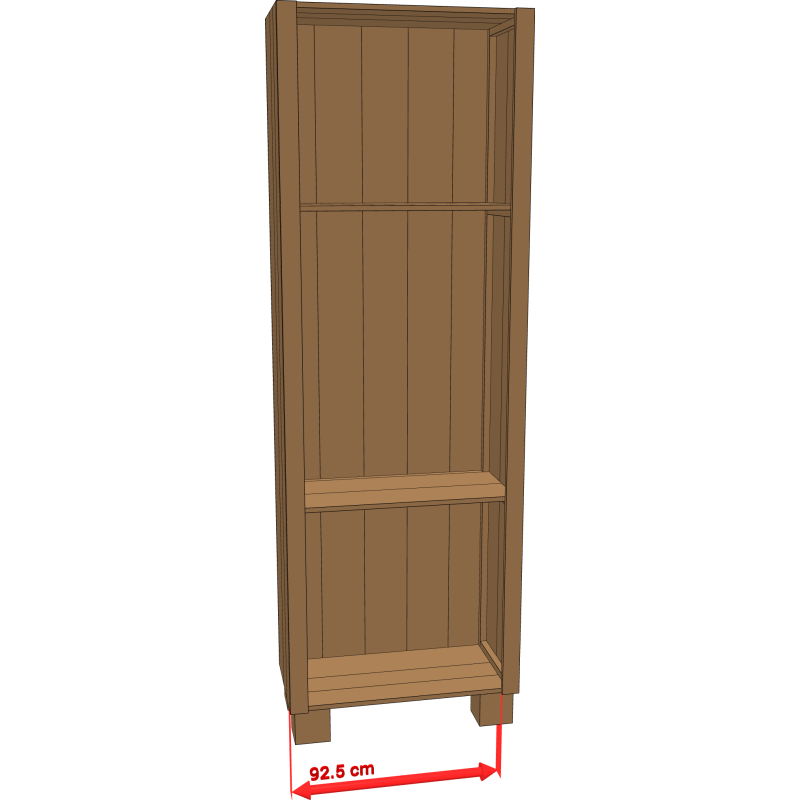
\includegraphics[width=0.8\textwidth]{scene 10 - deurpost a.png}
    \caption{Door frame global}
    \label{fig:stap 10a}
\end{figure}

\begin{figure}[h!]
    \centering
    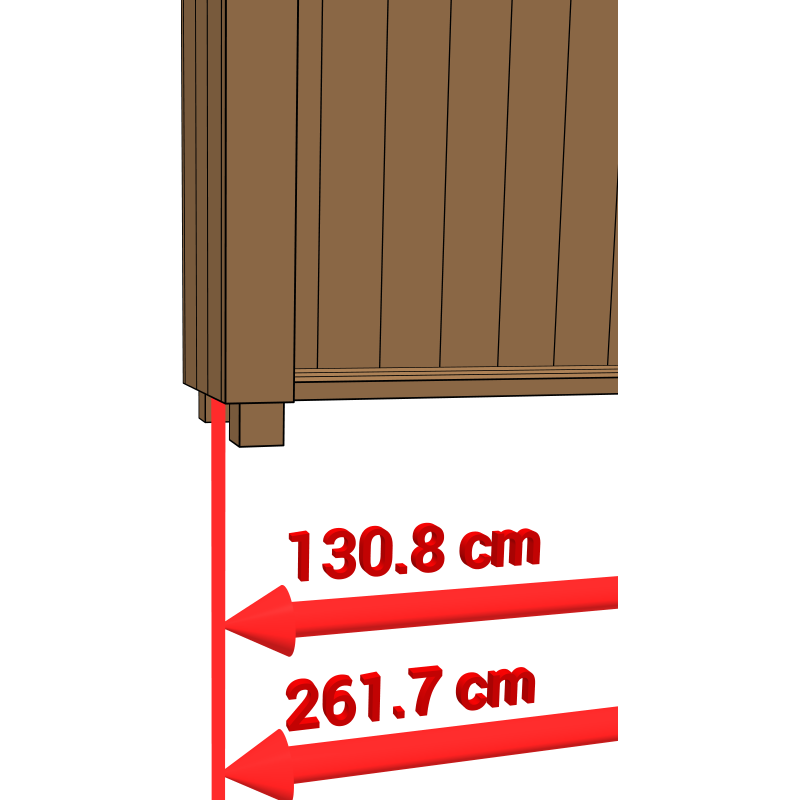
\includegraphics[width=0.8\textwidth]{scene 10 - deurpost b.png}
    \caption{Door frame local}
    \label{fig:stap 10b}
\end{figure}

\clearpage
\newpage

\subsection{Step 11 - Doors}

Then the doors of the cabinet are constructed. The table below shows the materials required for this step. With this list you create one door, repeat this step for the number of doors in your cabinet.

\begin{table}[h!]
\centering
\caption{Step 11 Door(s)}
\begin{tabular}{rrrr}
\toprule
 length &  width &  thickness &  ammount \\
\midrule
   90,0 &   20,0 &        2,0 &        3 \\
  295,0 &   14,7 &        2,0 &        2 \\
  295,0 &   20,0 &        2,0 &        3 \\
\bottomrule
\end{tabular}
\end{table}


The image below shows the height at which the \textbf{middle} of \textbf{both the horizontal shelves and the hinges} are attached to the other side. To fasten the planks, one screw per horizontal plank per vertical plank is used. For each hinge, 10 screws are taken into account. For this you use \textbf{screw 3} as indicated in table 4 of chapter 2.

The measurements are given relative to the bottom of the door. The image below is depicted extra large in the appendix.

\begin{figure}[h!]
    \centering
    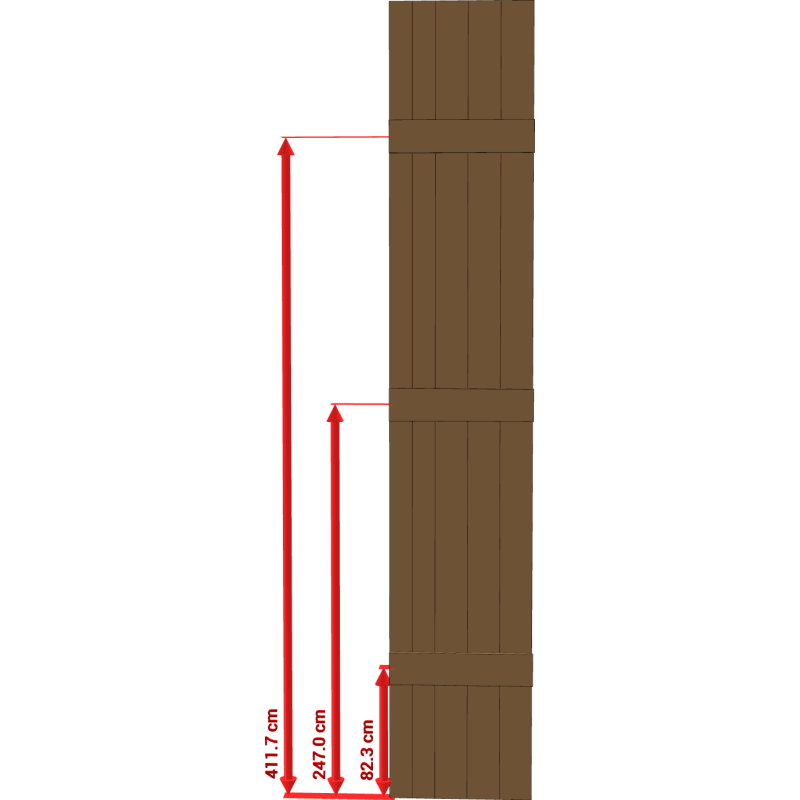
\includegraphics[width=0.8\textwidth]{scene 11 - deur.png}
    \caption{Door}
    \label{fig:stap 11}
\end{figure}

\clearpage
\newpage

\subsection{Step 12 - Complete cabinet}

Finally, the doors are attached to the cabinet. Here you can choose which side you want to place the hinges on. Once the doors are attached, the locks can be placed. The table below shows the materials required for this step.

\begin{table}[h!]
\centering
\caption{Stap 12 Scharnieren}
\begin{tabular}{rrrr}
\toprule
 lengte &  breedte &  dikte &  aantal \\
\midrule
    5,0 &     10,0 &    1,0 &       9 \\
   20,0 &      7,0 &    1,0 &       9 \\
\bottomrule
\end{tabular}
\end{table}


The image below shows an example of how the doors can be attached to the cabinet. To connect the hinges and locks use \textbf{screw 3} as indicated in table 4 of chapter 2. This screw first goes through the plank and then ends in the beam.

The images below are depicted extra large in the appendix.

\begin{figure}[h!]
    \centering
    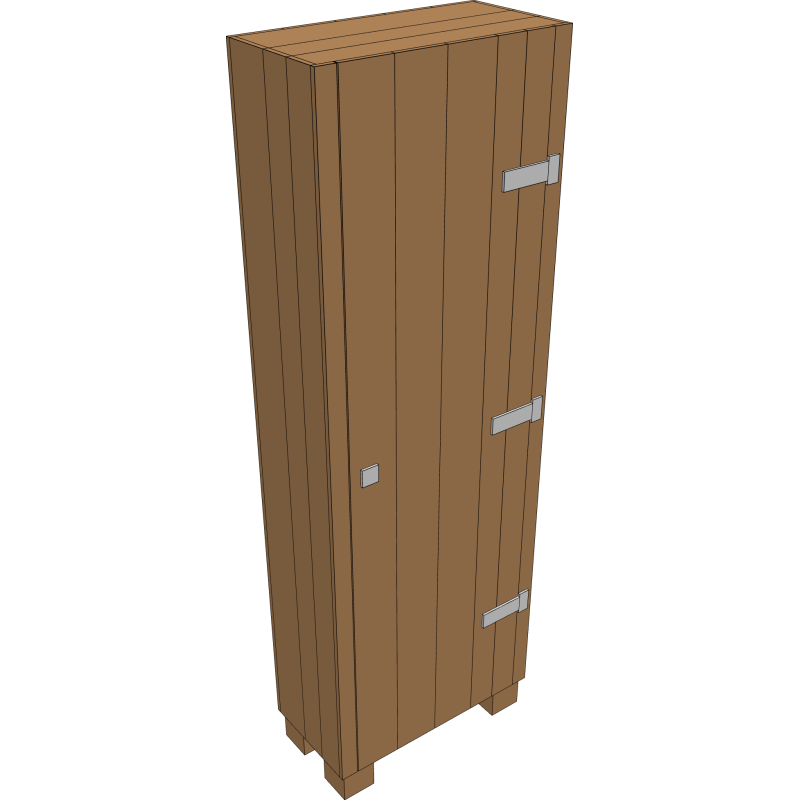
\includegraphics[width=0.8\textwidth]{scene 12 - compleet.png}
    \caption{Your new cabinet is ready to use!}
    \label{fig:stap 12}
\end{figure}

\clearpage
\newpage

\section{Appendix}

\begin{figure}[h!]
    \centering
    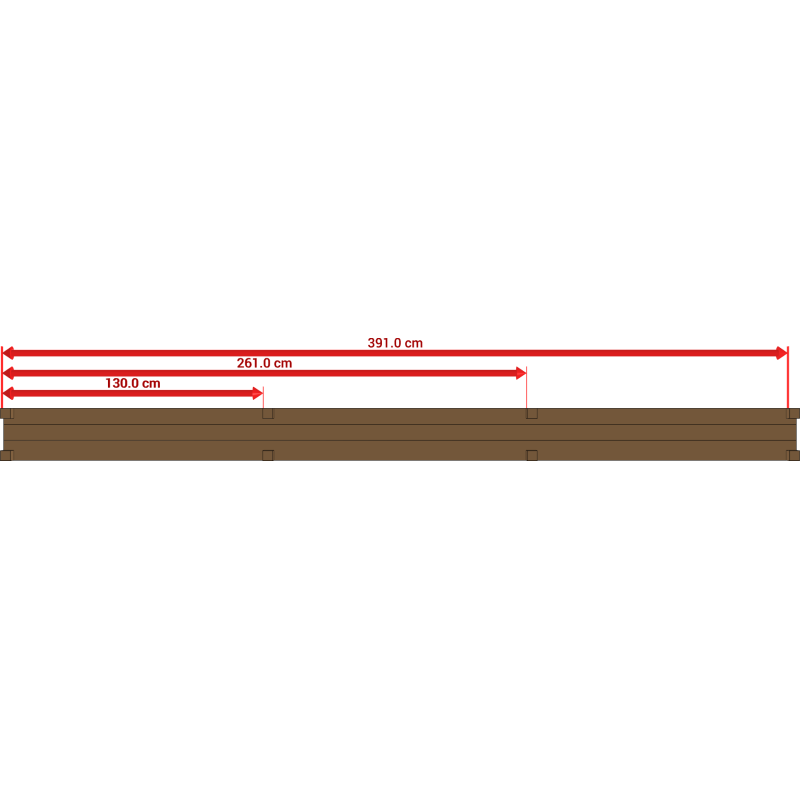
\includegraphics[width=\textwidth]{scene 1 - bottom.png}
    \caption{Bottom view cabinet}
\end{figure}

\begin{figure}[h!]
    \centering
    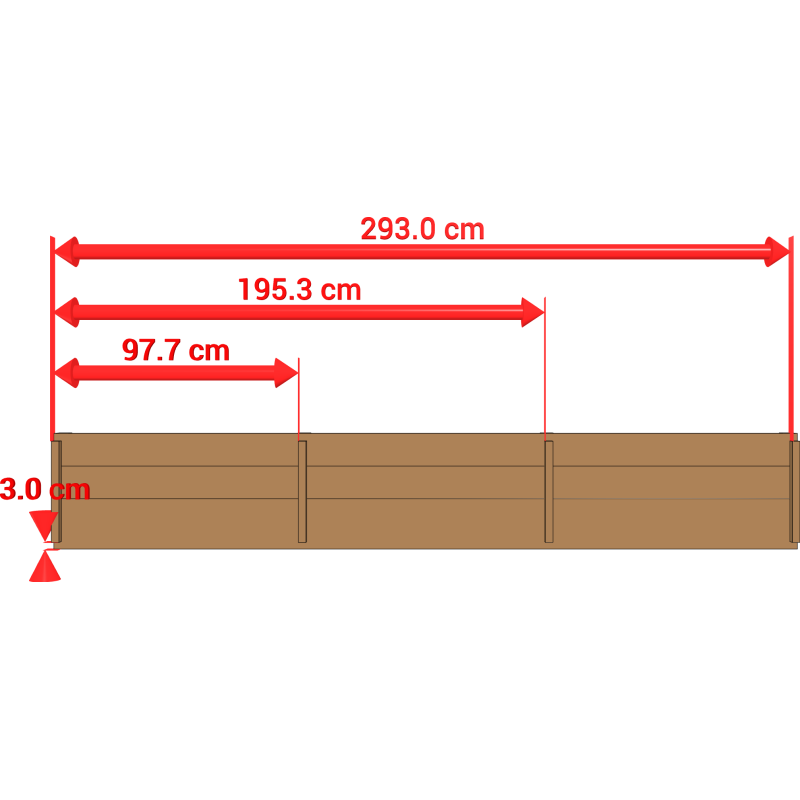
\includegraphics[width=\textwidth]{scene 2 - bottom rib.png}
    \caption{Ribs on cabinet}
\end{figure}

\begin{figure}[h!]
    \centering
    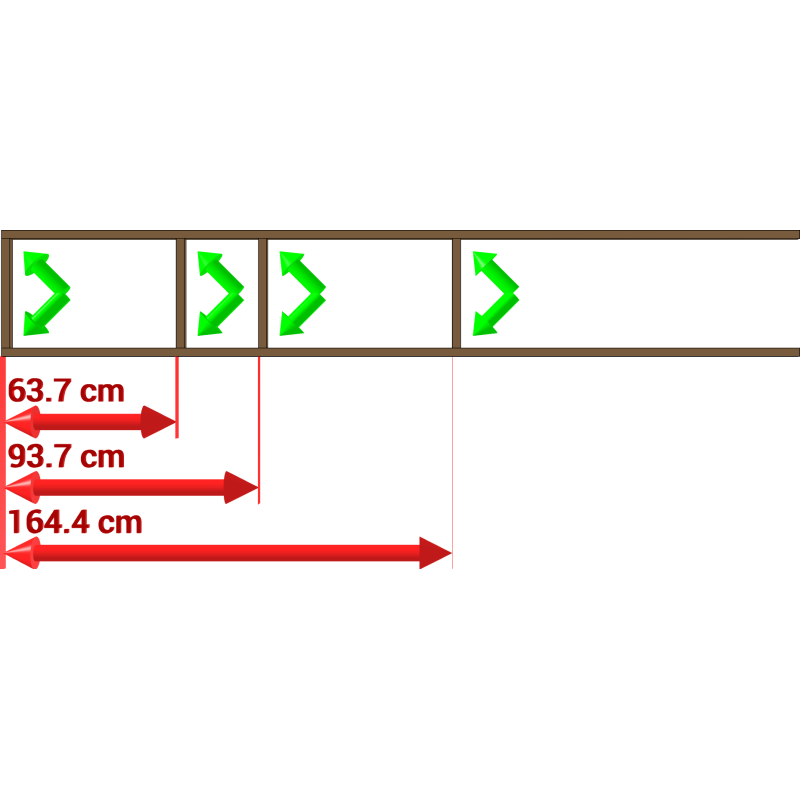
\includegraphics[width=\textwidth]{scene 3 - ladder.png}
    \caption{Ladder frame}
\end{figure}

\begin{figure}[h!]
    \centering
    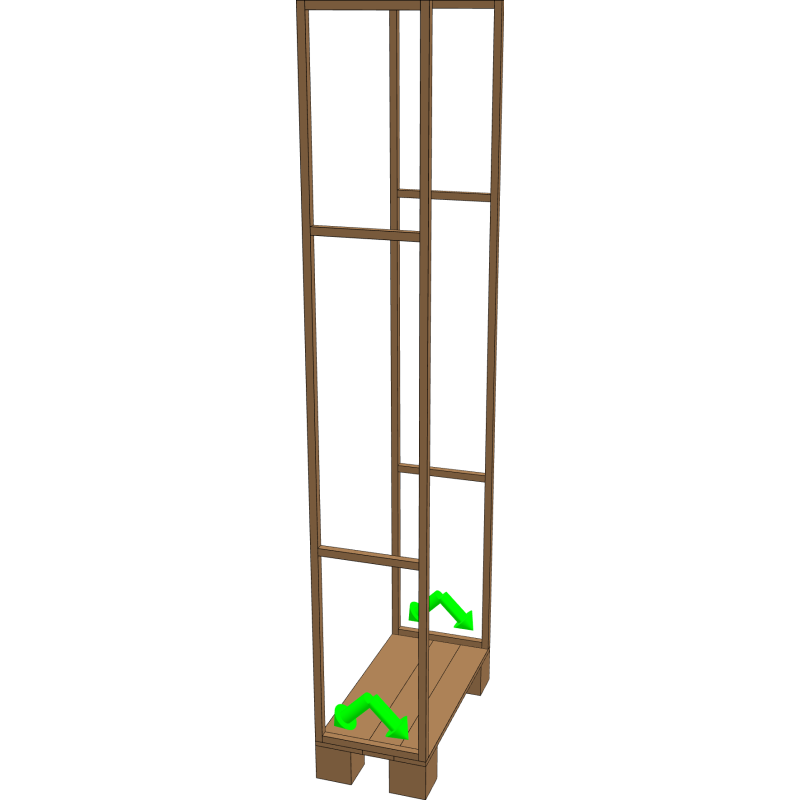
\includegraphics[width=\textwidth]{scene 4 - geraamte.png}
    \caption{Ladder frame on bottom}
\end{figure}

\begin{figure}[h!]
    \centering
    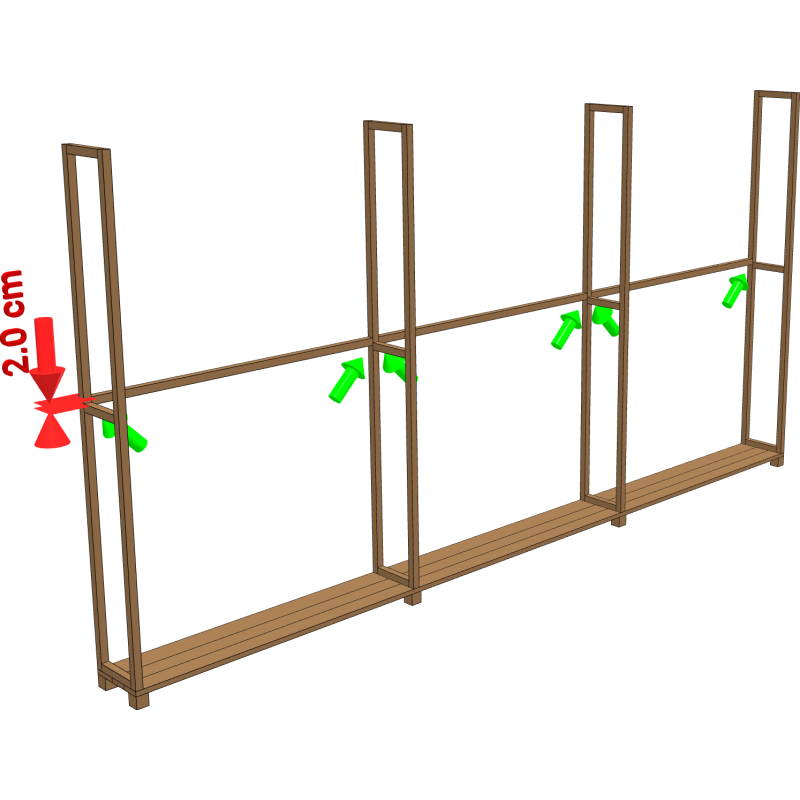
\includegraphics[width=\textwidth]{scene 5 - achterrib a.png}
    \caption{Backside rib global}
\end{figure}

\begin{figure}[h!]
    \centering
    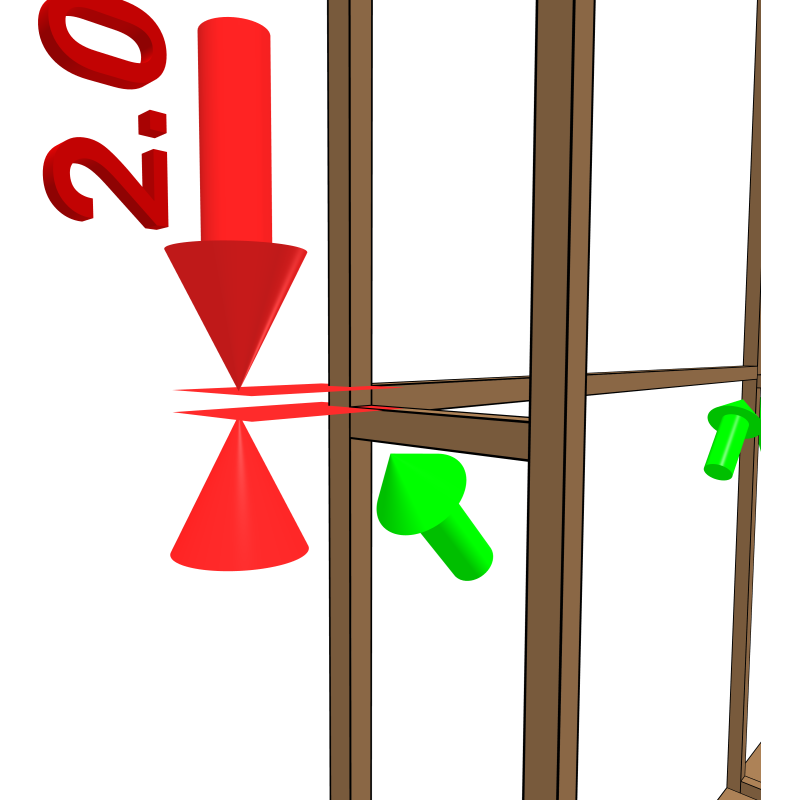
\includegraphics[width=\textwidth]{scene 5 - achterrib b.png}
    \caption{Backside rib local}
\end{figure}

\begin{figure}[h!]
    \centering
    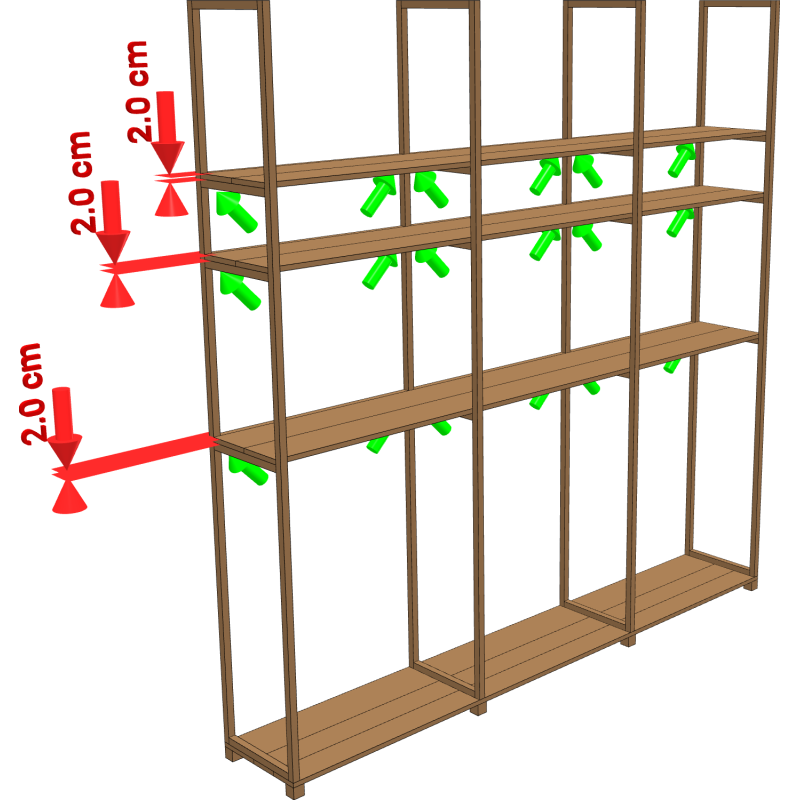
\includegraphics[width=\textwidth]{scene 6 - vlonders a.png}
    \caption{Decking global}
\end{figure}

\begin{figure}[h!]
    \centering
    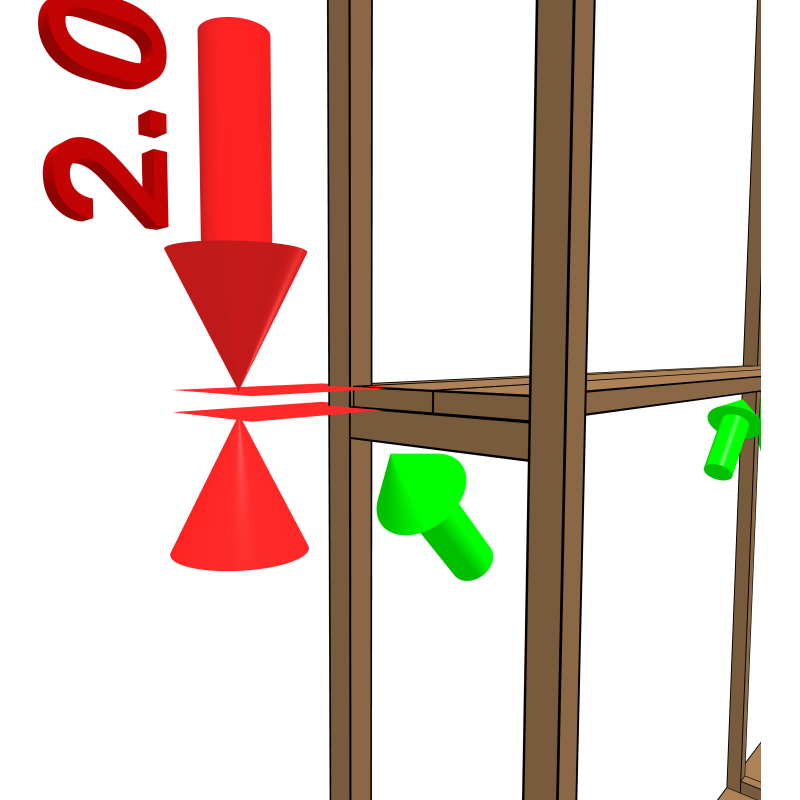
\includegraphics[width=\textwidth]{scene 6 - vlonders b.png}
    \caption{Decking local}
\end{figure}

\begin{figure}[h!]
    \centering
    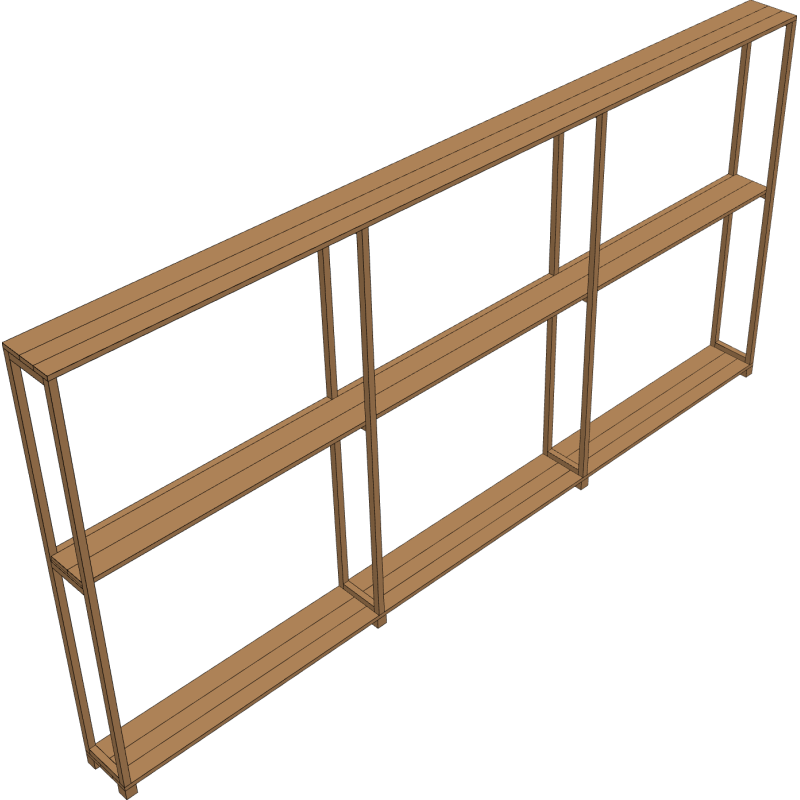
\includegraphics[width=\textwidth]{scene 7 - boven.png}
    \caption{Topside cabinet}
\end{figure}

\begin{figure}[h!]
    \centering
    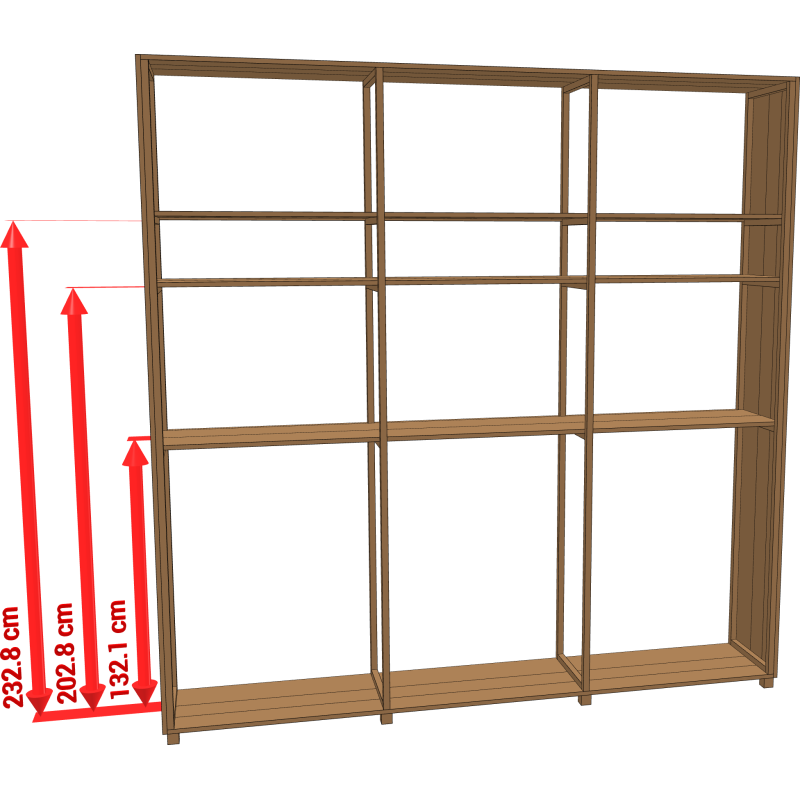
\includegraphics[width=\textwidth]{scene 8 - links_rechts.png}
    \caption{Sides cabinet}
\end{figure}

\begin{figure}[h!]
    \centering
    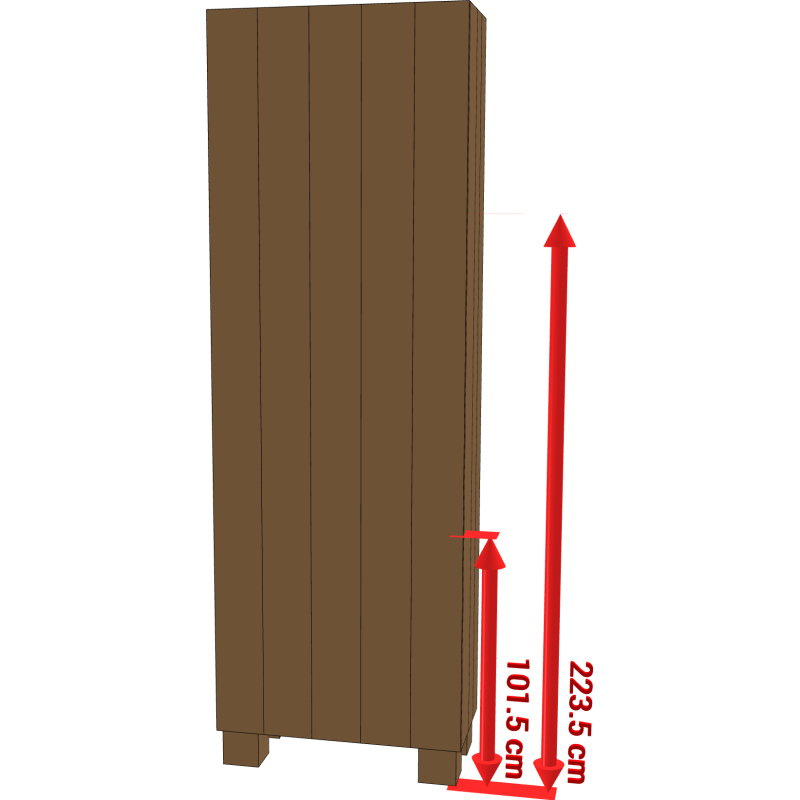
\includegraphics[width=\textwidth]{scene 9 - achterkant.png}
    \caption{Backside cabinet}
\end{figure}

\begin{figure}[h!]
    \centering
    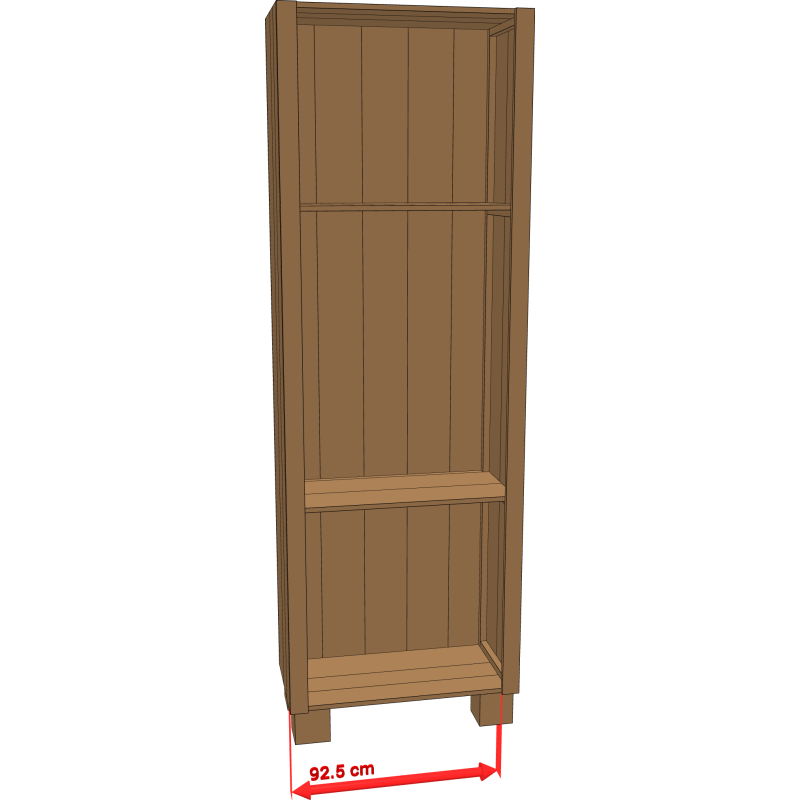
\includegraphics[width=\textwidth]{scene 10 - deurpost a.png}
    \caption{Door frame global}
\end{figure}

\begin{figure}[h!]
    \centering
    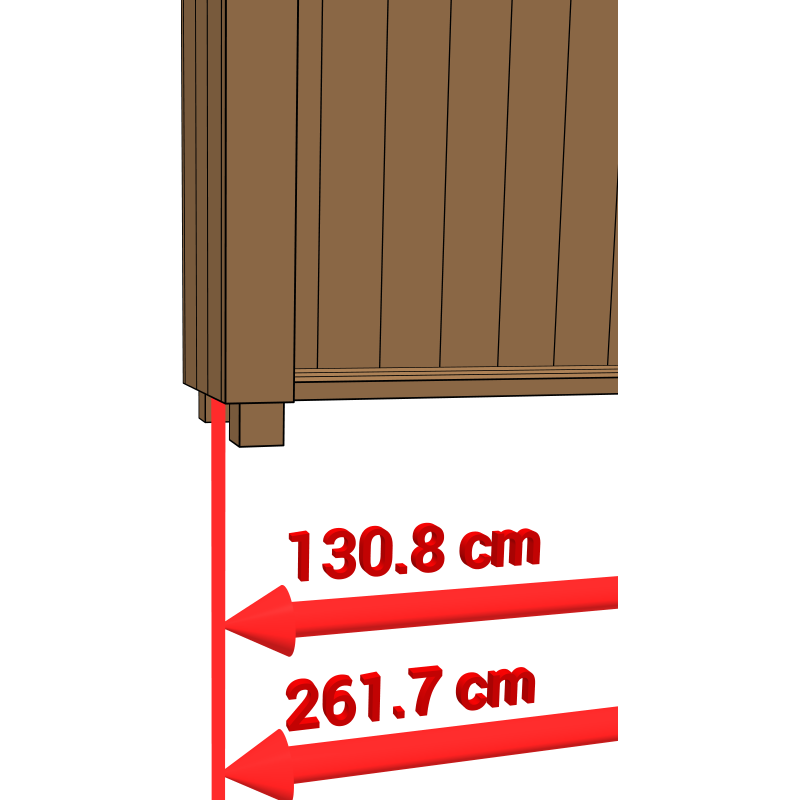
\includegraphics[width=\textwidth]{scene 10 - deurpost b.png}
    \caption{Door frame local}
\end{figure}

\begin{figure}[h!]
    \centering
    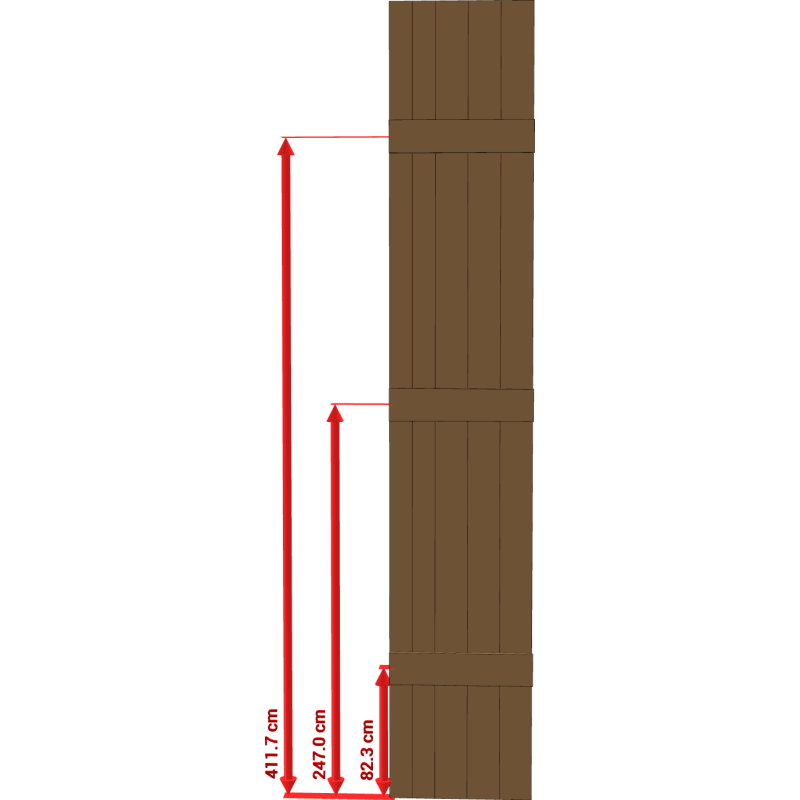
\includegraphics[width=\textwidth]{scene 11 - deur.png}
    \caption{Door}
\end{figure}

\begin{figure}[h!]
    \centering
    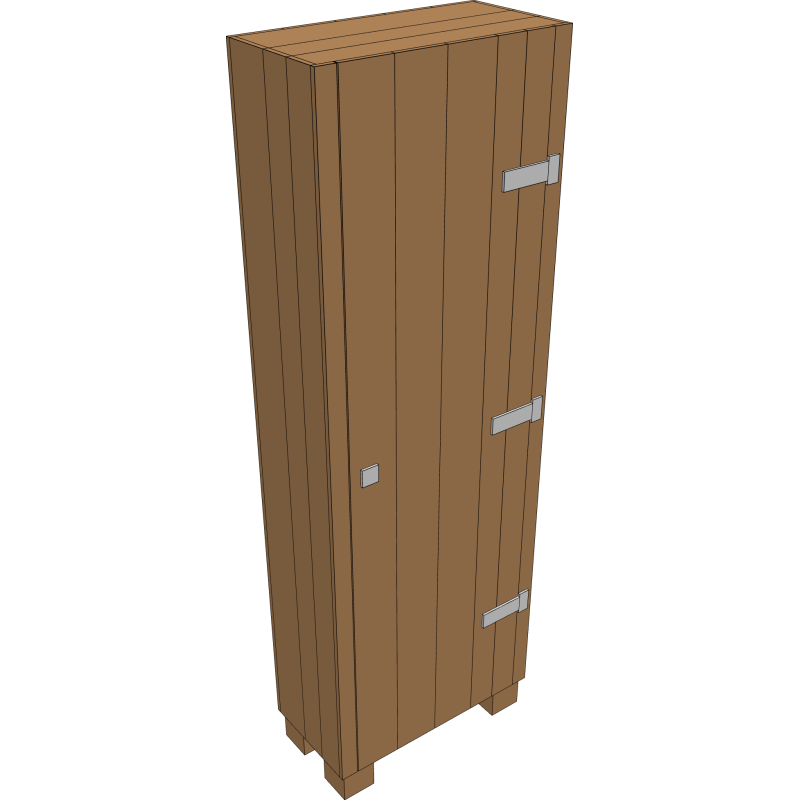
\includegraphics[width=\textwidth]{scene 12 - compleet.png}
    \caption{Your new cabinet is ready to use!}
\end{figure}

\end{document}